\section{CFPQ Full-Stack Support}

In order to provide full-stack support of CFPQ it is necessatry to choose an appropriate graph database.
It was shown by Arseniy Terekhov et al.~\cite{10.1145/3398682.3399163} that matrix-based algorithm can be naturally integrated into RedisGraph graph database because the algorithm and the database both operate over a matrix representation of graphs.
Moreover, RedisGraph supports Cypher as a query language and there is a proposal which describes Cypher extension for context-free constraints.
Thus we chose RedisGraph as a base for our solution.


\subsection{Cypher Extension}
\label{subsec:cypher-extension}

The first thing to do is to extend the Cypher parser to support the context-free constraints.
Tobias Lindaaker proposed an extension  for context free constraints to the Cypher syntax\footnote{\label{cypher-proposal}Formal syntax specification: \url{https://github.com/thobe/openCypher/blob/rpq/cip/1.accepted/CIP2017-02-06-Path-Patterns.adoc\#11-syntax}. Access date: 19.07.2020.}, which is not implemented in the Cypher parsers yet.

This extension introduces path patterns, which are a powerful alternative to the original Cypher relationship patterns.
Path patterns allow one to express regular constrains over the basic patterns such as relationship and node patterns.
Like relationship patterns, they can be specified in the \texttt{MATCH} clause.

The main feature which allows one to specify context-free constraints is \textit{named path patterns}: a path pattern can be assigned a name which can be used in other patterns or within the same pattern.
Named patterns can be defined in the \texttt{PATH PATTERN} clause.
Using this feature, the structure of queries is pretty similar to a context-free grammar in the Extended Backus-Naur Form (EBNF)~\cite{EBNF_ISO}.

\begin{algorithm}
\floatname{algorithm}{Listing}
\begin{algorithmic}[1]
\caption{Query based on the example grammar $G_1$ (eq.~\ref{eqn:g1_example}) written in Cypher with path patterns}
\label{lst:cypher_example}
\State PATH PATTERN S = ()-/ [:c $\sim$S :d] | [:c (:y) :d] /->()
\State MATCH (v:x)-[:a | :c]->()-/ :b $\sim$S /->(to)
\State RETURN v, to
\end{algorithmic}
\end{algorithm}


An example of a query which uses named path patters is presented in listing~\ref{lst:cypher_example}.
This query is based on the context-free grammar $G_1$ (eq.~\ref{eqn:g1_example}).
Namely, the path pattern named \texttt{S} specifies exactly the same constraint as the grammar $G_1$.
The \texttt{MATCH} clause consists of the relation pattern \texttt{[:a | :c]} and the path pattern \texttt{/:b $\sim$S/}, and this path pattern references the named pattern \texttt{S}.
The constraint specifies that a path of interest starts in a vertex labelled \texttt{x}, goes through an edge labelled either \texttt{a} or \texttt{c}, then the rest of the path is constrainted by a path pattern which starts with an edge \texttt{b} and follows with a path matched with \texttt{S}.
The \texttt{RETURN} clause specifies what the result of the query is supposed to be.
For the example graph $D_1$, this query returns the set of vertex pairs $\{(0, 4), (0, 5)\}$.

RedisGraph database supports a subset of the Cypher language and uses \texttt{libcypher-parser}\footnote{The \texttt{libcypher-parser} is an open-source parser library for Cypher query language. GitHub repository of the project: \url{https://github.com/cleishm/libcypher-parser}. Access date: 19.07.2020.} library to parse queries.
We extend this library with the new syntax described in the proposal.
Note that we implement\footnote{The modified libcypher-parser library with support of syntax for path patterns: \url{https://github.com/YaccConstructor/libcypher-parser}. Access date: 19.07.2020.} the complete syntax extension, not only the part necessary for simple CFPQ.

\subsection{RedisGraph Extension}

As a proof-of-concept, we implemented the multiple-source algorithm in the RedisGraph backend.
We partially supported the proposed syntax extension in RedisGraph query execution engine so that one can specify the labels of edges and vertices and use named path patterns.

Processing the input as a whole may require a lot of memory.
RedisGraph implements lazy evaluation: it creates execution strategy in terms of elementary operations each of which processes the input sequentially in \emph{chunks}.
This reduces memory consumption so that it does not depend on the input size which is crucial when dealing with big real-world graphs.
However processing chunks comes with a time overhead.
By changing the size of a chunk, a developer may adjust the ratio between the time and memory consumption so that it fits their needs.

We use subsets of the start vertices as chunks since it is most natural in the multiple source algorithm.
We study how the size of a chunk affects the performance in the evaluation.

\subsection{Evaluation}

In order to demonstrate the applicability of the implemented extension for RedisGraph we evaluate it on the subset of cases provided in the section~\ref{sect:py_algo_evaluation}.

For RedisGraph evaluation, we used a PC with Ubuntu 18.04 installed.
It has Intel Core i7-6700 CPU, 3.4GHz, and DDR4 64Gb RAM.
RedisGraph with our extensions is installed from the GitHub repository\footnote{Sources of RedisGraph database with full-stack CFPQ support:\url{https://github.com/YaccConstructor/RedisGraph/tree/path_patterns_dev}. Access data: 19.07.2020.}.

\subsubsection{Data Preparation}

We use the same graphs which are presented in table~\ref{tbl:graphs_for_cfpq} to evaluate RedisGraph-based solution.

Graphs are loaded into the RedisGraph database so that each vertex has a unique property \verb|id| in the range $[0 \ldots |V|-1]$, where $|V|$ is a number of vertices in the graph to load.
This allows us to generate queries for start vertex set with specific size using templates.
%\simpleton{(here chunk size don`t means "chunk size parameter of RedisGraph". But "chunk size parameter of RedisGraph" in experiments such enough to evaluate multiple source algorithm only single time)}.
The template for the $g_1$ query is provided in listing~\ref{lst:query_pattern_g1}.
Here \texttt{\{id\_from\}} and \texttt{\{id\_to\}} are placeholders for the lower and the upper bounds for \verb|id|.
The example of the concrete query for the start set of size 16 is presented in listing~\ref{lst:query_g1}.

\begin{algorithm}
\floatname{algorithm}{Listing}
\begin{algorithmic}[1]
\caption{Cypher query pattern for $g_1$}
\label{lst:query_pattern_g1}
\State PATH PATTERN S =  \par
 \hskip\algorithmicindent ()-/ [<:SubClassOf [$\sim$S | ()] :SubClassOf] \par
 \hskip\algorithmicindent | [<:Type [$\sim$S | ()] :Type] /->()
\State MATCH (src)-/ $\sim$S /->()
\State WHERE \{id\_from\} <= src.id and src.id <= \{id\_to\}
\State RETURN count(*)
\end{algorithmic}
\end{algorithm}

\begin{algorithm}
\floatname{algorithm}{Listing}
\begin{algorithmic}[1]
\caption{Query $g_1$ in Cypher using template from listing~\ref{lst:query_pattern_g1}}
\label{lst:query_g1}
\State PATH PATTERN S =  \par
 \hskip\algorithmicindent ()-/ [<:SubClassOf [$\sim$S | ()] :SubClassOf] \par
 \hskip\algorithmicindent | [<:Type [$\sim$S | ()] :Type] /->()
\State MATCH (src)-/ $\sim$S /->()
\State WHERE 15 <= src.id and src.id <= 31
\State RETURN count(*)
\end{algorithmic}
\end{algorithm}

We implemented a query generator for the queries $g_1$ and $geo$ to create concrete queries for all the start sets which are used in the previous experiment.


\subsubsection{Evaluation Results}

We use $geo$ query for \textit{geospecies} graph as one of the hardest queries, and $g_1$ query for other graphs.
We measure time and memory consumption for each start set.
The results are presented in figures~\ref{fig:redis_core_all}--\ref{fig:redis_gohierarchy_all}.

\begin{figure}[h]
\centering
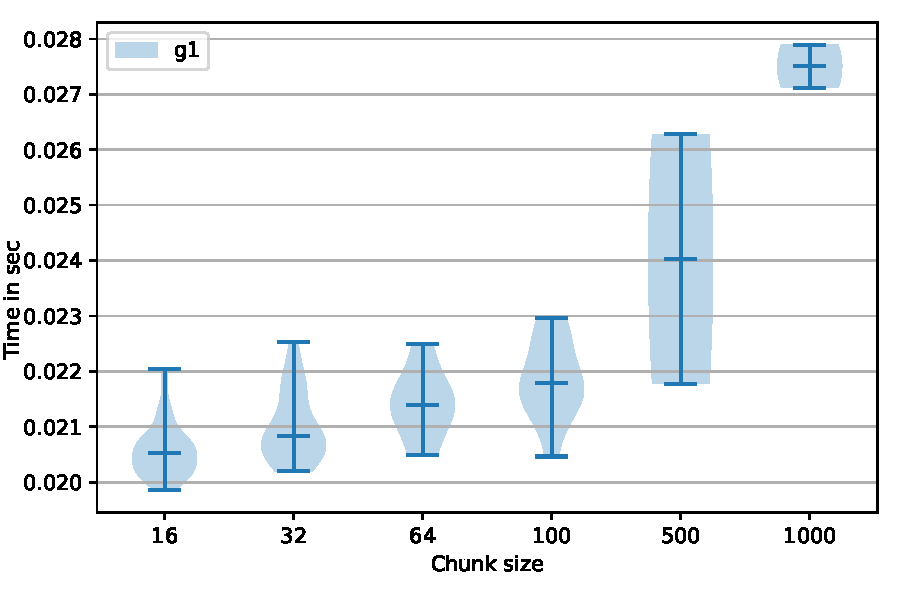
\includegraphics[width=0.45\textwidth]{data/raw_redis/core.pdf}
\caption{RedisGraph performance on \textit{core} graph}
\label{fig:redis_core_all}
\end{figure}


\begin{figure}[h]
\centering
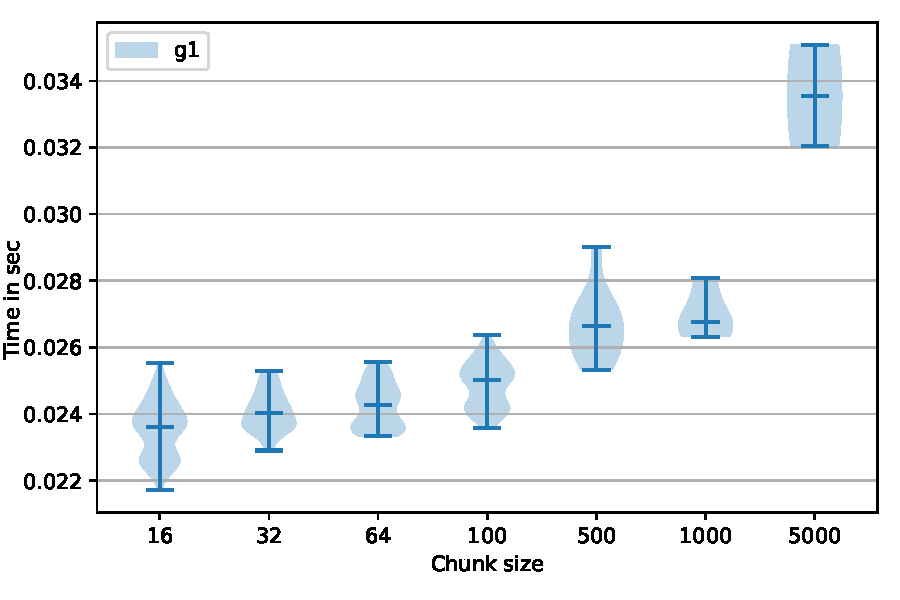
\includegraphics[width=0.45\textwidth]{data/raw_redis/pathways.pdf}
\caption{RedisGraph performance on \textit{pathways} graph}
\label{fig:redis_pathways_all}
\end{figure}

\begin{figure}[h]core
\centering
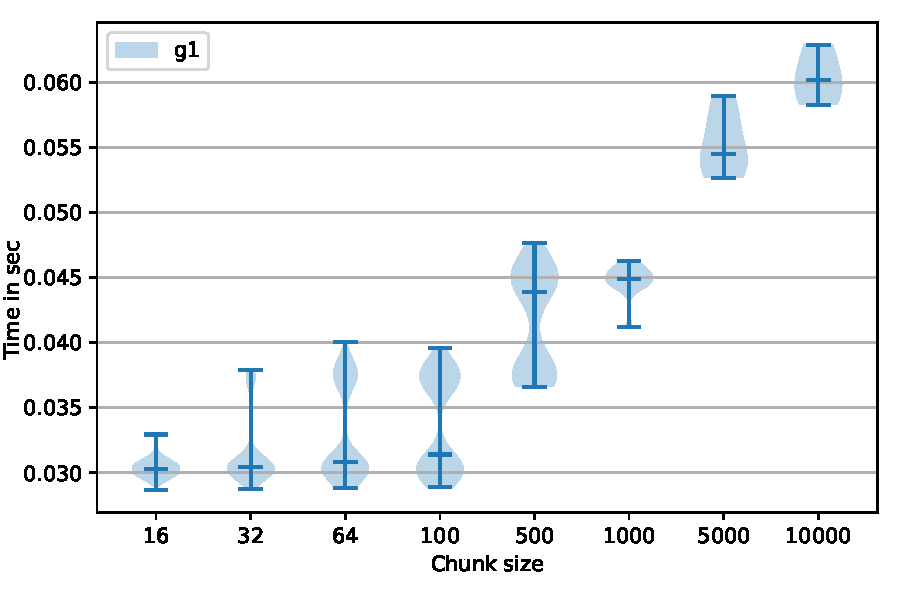
\includegraphics[width=0.45\textwidth]{data/raw_redis/enzyme.pdf}
\caption{RedisGraph performance on \textit{enzyme} graph}
\label{fig:redis_enzyme_all}
\end{figure}


\begin{figure}[h]
\centering
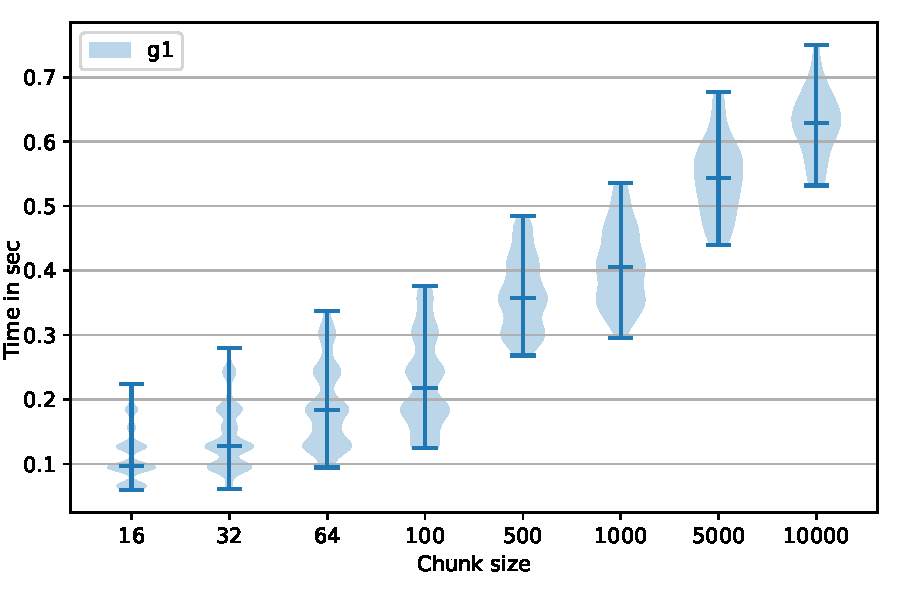
\includegraphics[width=0.45\textwidth]{data/raw_redis/go.pdf}
\caption{RedisGraph performance on \textit{go} graph}
\label{fig:redis_go_all}
\end{figure}

\begin{figure}[h]
\centering
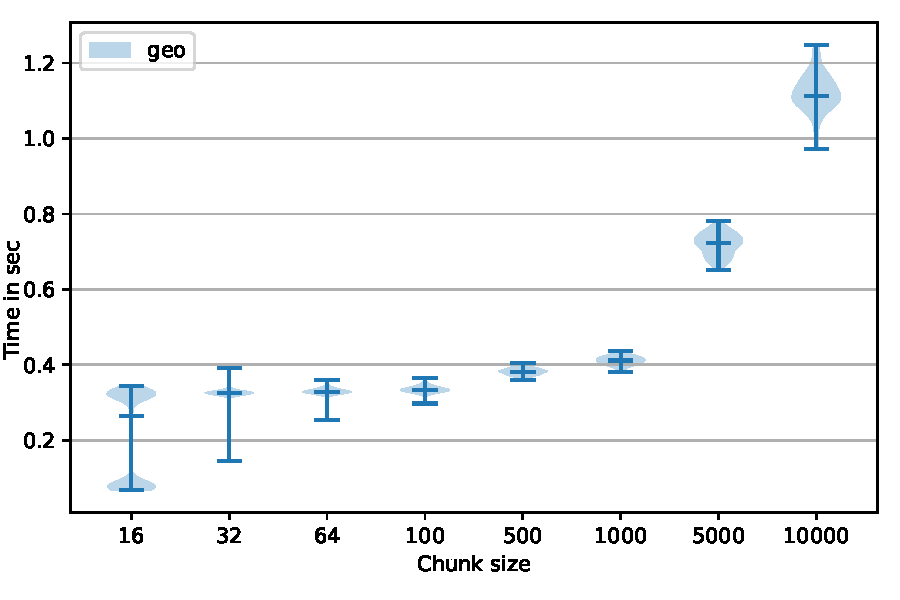
\includegraphics[width=0.45\textwidth]{data/raw_redis/geospecies.pdf}
\caption{RedisGraph performance on \textit{geospecies} graph}
\label{fig:redis_geospecies_all}
\end{figure}

\begin{figure}[h]
\centering
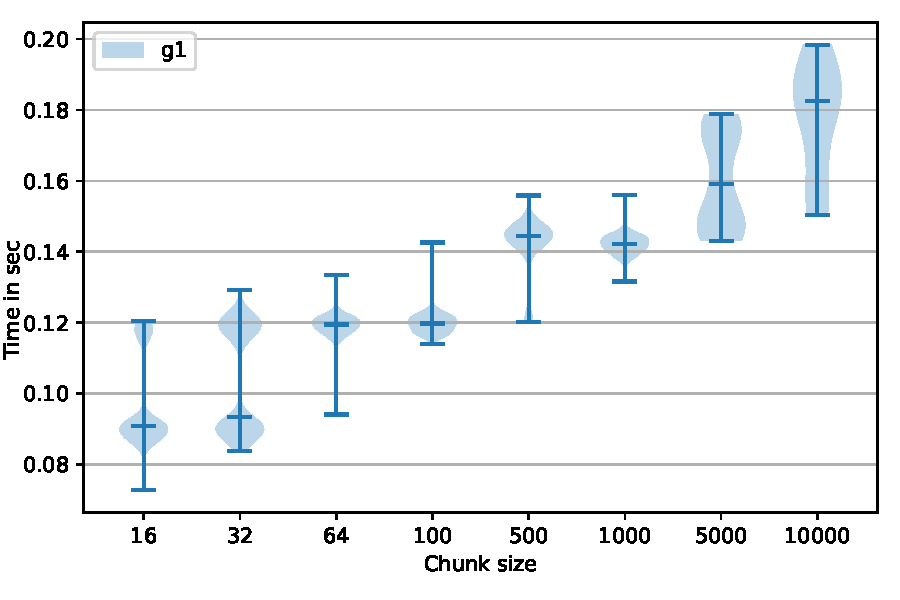
\includegraphics[width=0.45\textwidth]{data/raw_redis/eclass_514en.pdf}
\caption{RedisGraph performance on \textit{eclass\_514en} graph}
\label{fig:redis_eclass_all}
\end{figure}

\begin{figure}[h]
\centering
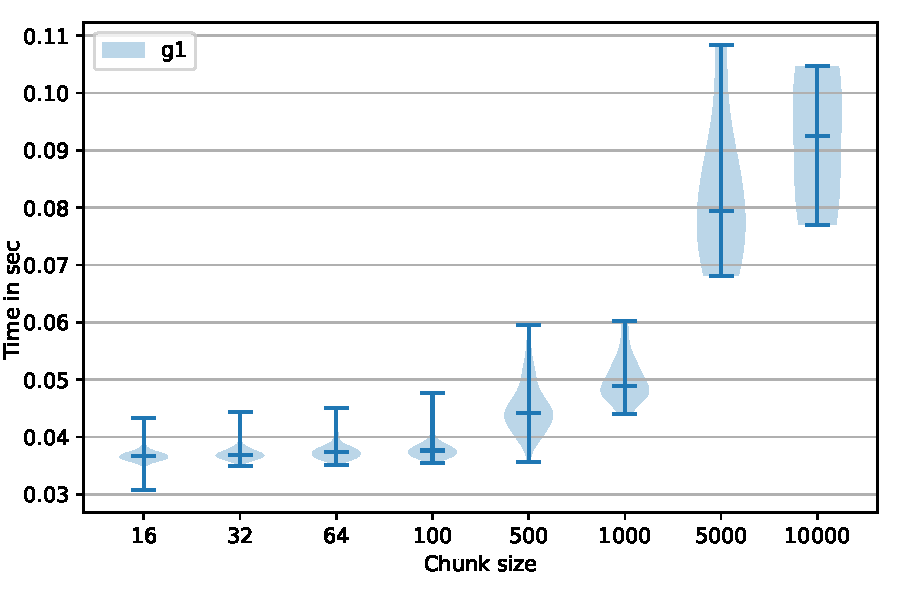
\includegraphics[width=0.45\textwidth]{data/raw_redis/gohierarchy.pdf}
\caption{RedisGraph performance on \textit{gohierarchy} graph}
\label{fig:redis_gohierarchy_all}
\end{figure}

We can see, that the execution time is comparable with the results of the previous experiment presented in section~\ref{sect:py_algo_evaluation}.
The execution time for all sets, except the set of size 10~000 for \textit{geospecies} graph (fig.~\ref{fig:redis_geospecies_all}) is less then 1 second.
Moreover, for sets of size 16, processing median time is less then 0.1 second, except for \textit{geospecies} graph.

Memory consumption for the big graphs \textit{eclass\_514en} and \textit{geospecies} is presented in figures~\ref{fig:redis_memory_eclass} and~\ref{fig:redis_memory_geospecies} respectively.
The amount of memory used depends on the graph and the query, but RedisGraph uses less that 50Mb of RAM to process one set for relatively small sets ($\leq 1000$).
Note that RedisGraph includes memory management system, thus we measured all allocated memory, not only the memory really used for the query evaluation.
As a result, we can conclude that the multiple-source CFPQ is significantly more memory efficient than creation of the complete reachability index and its filtering: processing the set of size 10~000 on \textit{geospecies} graph requires less than 200Mb, while full index creation requires 16Gb~\cite{10.1145/3398682.3399163}.

\begin{figure}[h]
\centering
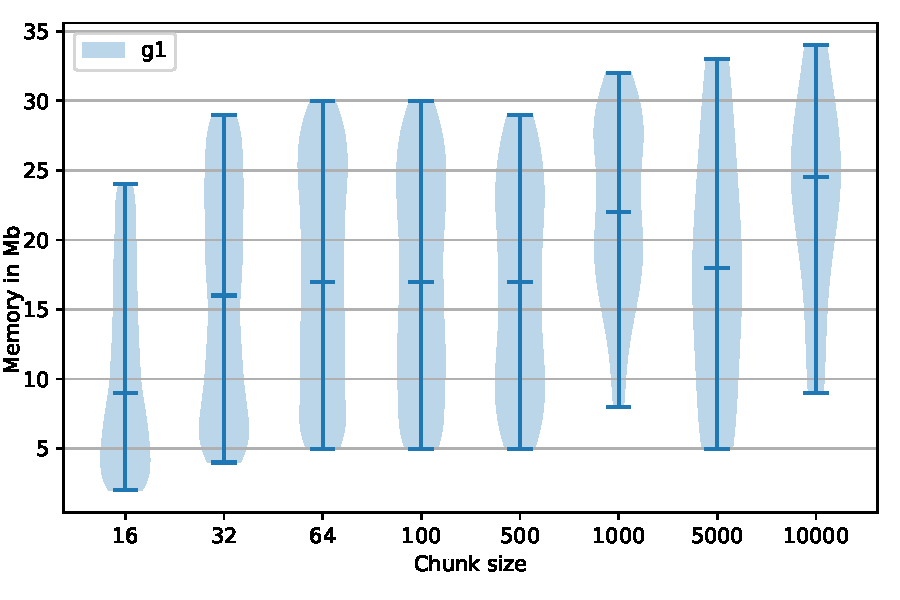
\includegraphics[width=0.5\textwidth]{data/raw_memory/eclass_514en.pdf}
\caption{RedisGraph memory consumption on \textit{eclass\_514en} graph}
\label{fig:redis_memory_eclass}
\end{figure}

\begin{figure}[h]
\centering
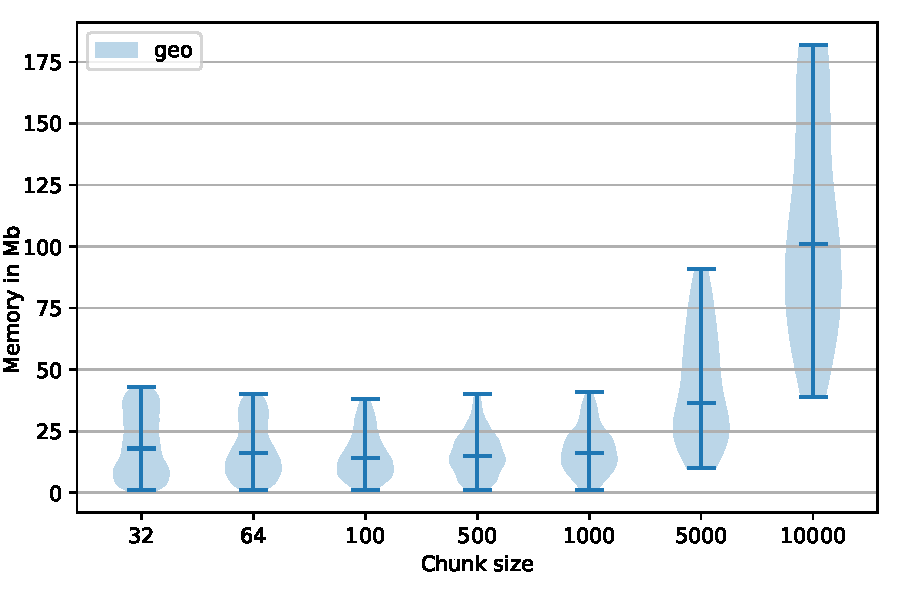
\includegraphics[width=0.5\textwidth]{data/raw_memory/geospecies.pdf}
\caption{RedisGraph memory consumption on \textit{geospecies} graph}
\label{fig:redis_memory_geospecies}
\end{figure}


\begin{algorithm}
\floatname{algorithm}{Listing}
\begin{algorithmic}[1]
\caption{Query $g_1$ in Cypher for all-pairs scenario evaluation}
\label{lst:query_g1_full}
\State PATH PATTERN S =  \par
 \hskip\algorithmicindent ()-/ [<:SubClassOf [$\sim$S | ()] :SubClassOf] \par
 \hskip\algorithmicindent | [<:Type [$\sim$S | ()] :Type] /->()
\State MATCH ()-/ $\sim$S /->()
\State RETURN count(*)
\end{algorithmic}
\end{algorithm}

We also evaluate how the chunk size affects the performance on the all-pairs reachability problem.
We fix the size of a chunk to be 1000 for graphs of different sizes and measure time and memory required to process queries.
Namely, we evaluate the query, presented in listing~\ref{lst:query_g1_full}.
It is similar to the query from the previous scenario, but it does not constraint  vertices ids (it does not have the \texttt{WHERE} clause).
We measure total processing time (in seconds) and total required memory (in Mb).
Also, we compare our solution with the results of Arseniy Terekhov et al. from~\cite{10.1145/3398682.3399163} in which the Azimov's algorithm was naively integrated with RedisGraph without support of lazy query evaluation and query language.
Similar hardware and the same input graphs and queries were used.
Results are provided in table~\ref{tbl:redis_full_graph_processing}.

{\setlength{\tabcolsep}{0.25em}
\begin{table}
{
\caption{Full graph processing time by RedisGraph with chunks of size 1000, time is measured in seconds, memory in Mb (\textbf{Chunks} --- the proposed solution, \textbf{Mono} --- results from~\cite{10.1145/3398682.3399163})}
\label{tbl:redis_full_graph_processing}
\small
\rowcolors{3}{black!2}{black!10}
\begin{tabular}{|l|c|c|c|c|c|c|}
\hline
\multirow{2}{*}{Graph} & \multirow{2}{*}{\#V} & \multirow{2}{*}{\#E} & \multirow{2}{*}{Query} & \multicolumn{2}{c|}{Chunks}  &  \multirow{2}{*}{Mono}  \\
                       &                      &                      &                        & Time   & Mem & \\
\hline
\hline
core                   & 1323                 & 4342                 & $g_1$                  & 0.003  & 2                  &  0.004 \\
pathways               & 6238                 & 18 598               & $g_1$                  & 0.031  & 6                  &  0.011 \\
gohierarchy            & 45 007               & 980 218              & $g_1$                  & 0.847  & 62                  &  0.091 \\
enzyme                 & 48 815               & 109 695              & $g_1$                  & 0.698  & 13                  &  0.018 \\
eclass\_514en          & 239 111              & 523 727              & $g_1$                  & 18.825 & 35                   &  0.067 \\
geospecies             & 450 609              & 2 311 461            & $geo$                  & 80.979 & 196                  &  7.146 \\
go                     & 272 770              & 534 311              & $g_1$                  & 72.034 & 40                  &  0.604 \\
\hline
\end{tabular}
}
\end{table}
}

Although chunk-by-chunk processing is slower, it still requires reasonable time.
Moreover, if the chunk size is comparable with the graph size (\textit{core} and \textit{pathways} graphs), then the execution time is comparable with the monolithic processing.
Thus one can decrease execution time by increasing the chunk size.
On the other hand, even with relatively small chunks (\textit{eclass\_514}, \textit{go} and \textit{geospecies} graphs), when for chunk-by-chunk processing is 100 times slower, our results are still reasonable for some cases.
For example, it requires more than 70 times less time for \textit{geospecies} graph processing than the solution of Jochem Kuijpers et al.~\cite{Kuijpers:2019:ESC:3335783.3335791} which is based on Neo4j and requires more than 6000 seconds.
Moreover, while the solution from~\cite{10.1145/3398682.3399163} requires huge amount of memory (more than 16Gb for \textit{geospecies} graph and $geo$ query), our solution requires only 196Mb.
We argue, that our solution is more suitable for general-purpose graph databases.
First of all, the core scenario when the set of start vertices is relatively small can be handled efficiently.
Second, all-pairs reachability, which is not a massive case, can be solved in reasonable time with low memory consumption.
One can easily tune our solution to get the optimal time and memory consumption for their specific case.

Finally, we conclude that the provided solution is a promising way to implement CPFQ for real-world graph databases.

